\documentclass[a4paper,12pt]{scrartcl}
\usepackage[ngerman]{babel}
\usepackage[utf8]{inputenc}
\usepackage[T1]{fontenc}
\usepackage{lmodern}
\usepackage{amssymb}
\usepackage{graphicx}
\usepackage{float}
\usepackage{amsmath}
\usepackage{multicol}
\usepackage{enumerate}
\usepackage{verbatim}
\usepackage{pgfplots}
\usepackage{scrpage2}\pagestyle{scrheadings}
\usepackage{tikz}
\usetikzlibrary{patterns}

\newcommand{\titleinfo}{Visualisierung und Diskussion}

\title{\titleinfo}
\author{Sönke Kracht, Sven-Hendrik Haase}
\date{\today}
\chead{\titleinfo}
\ohead{\today}
\setheadsepline{1pt}
\setcounter{secnumdepth}{0}
\newcommand{\qed}{\quad \square}

\begin{document}
\maketitle
\notag

\section{Jacobi}
\subsection{3 Prozesse, 2 Knoten}
\begin{figure}[H]
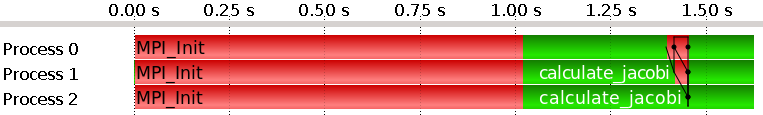
\includegraphics[scale=0.8]{jacobi-3-2-start.png}
\caption{Beginn des Programms}
\end{figure}

Das MPI\_Init verbraucht hier um die 1 Sekunde pro Prozess.

\begin{figure}[H]
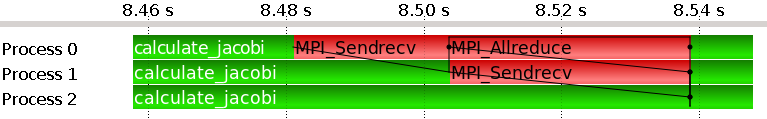
\includegraphics[scale=0.8]{jacobi-3-2-sync.png}
\caption{Sync-Übersicht}
\end{figure}

Aufällig ist die Treppenstruktur, die vom MPI\_Sendrecv verursacht wird. Dies 
ist vermutlich darauf zurückzuführen, dass wir Prozesse mit geradem 
und ungeradem Rang gleich behandelt haben. Das MPI\_Allreduce ist im ersten
Prozess nur so deutlich zu sehen, da er auf 
die Sendrecvs der anderen Prozesse warten muss.

\begin{figure}[H]
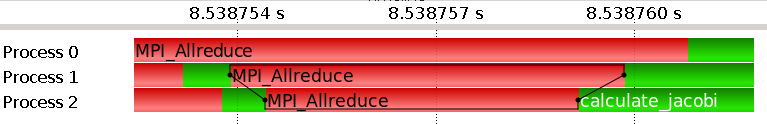
\includegraphics[scale=0.8]{jacobi-3-2-sync2.png}
\caption{Closeup vom Ende des Sync}
\end{figure}

Wie man an der Skala sieht, verbraucht das MPI\_Allreduce nach Ende des
Sendrecvs kaum noch Laufzeit. Ungünstig in unserem Programm ist, dass das 
MPI\_Allreduce auch bei Abbruch nach Iteration in jedem Durchlauf 
ausgeführt wird.

\begin{figure}[H]
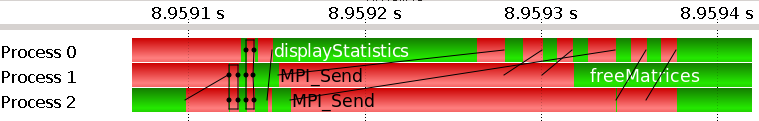
\includegraphics[scale=0.8]{jacobi-3-2-end.png}
\caption{Ende des Programms}
\end{figure}

Man sieht, wie der Hauptprozess die Matrix einsammelt, dies nimmt
überraschend wenig Zeit in Anspruch.

\subsection{5 Prozesse, 4 Knoten}
\begin{figure}[H]
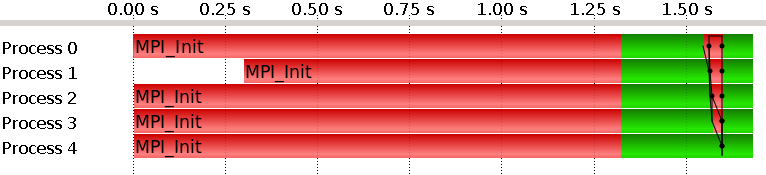
\includegraphics[scale=0.8]{jacobi-5-4-start.png}
\caption{Beginn des Programms}
\end{figure}
Das MPI\_Init verbraucht hier um die 1.25 Sekunden pro Prozess. Bei Process 1
fängt es etwas später an, was damit zu tun haben kann, dass einige Knoten zu
Schlafen beginnen, wenn sie länger nicht benutzt werden. Es kann auch damit zu
tun haben, dass in diesem Fall 2 Prozesse auf dem gleichen Knoten ausgeführt
werden.

\begin{figure}[H]
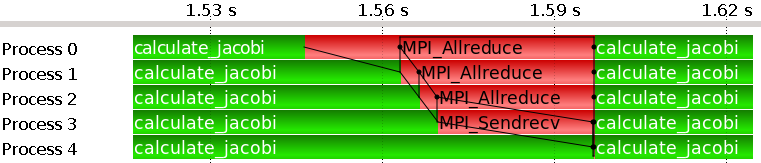
\includegraphics[scale=0.8]{jacobi-5-4-sync.png}
\caption{Sync-Übersicht}
\end{figure}

Man kann alle oben erwänten Phänomene in größerem Maßstab betrachten.

\begin{figure}[H]
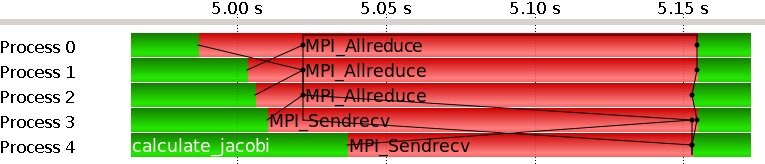
\includegraphics[scale=0.8]{jacobi-5-4-sync2.png}
\caption{Anomalie}
\end{figure}

Diese trat nur ein Mal in allen Programmdurchläufen auf. Die Kommunikation
dauert in diesem Fall in etwa vierfach so lange.

\begin{figure}[H]
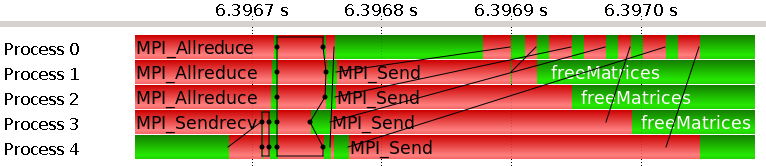
\includegraphics[scale=0.8]{jacobi-5-4-end.png}
\caption{Ende des Programms}
\end{figure}

\section{Gauss-Seidel}
\subsection{3 Prozesse, 2 Knoten}
\begin{figure}[H]
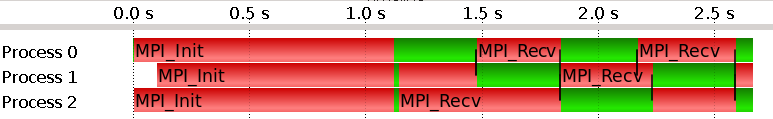
\includegraphics[scale=0.8]{gaussseidel-3-2-start.png}
\caption{Beginn des Programms}
\end{figure}
Das MPI\_Init verbraucht hier um die 1.15 Sekunden pro Prozess. Bei Process 1
fängt es etwas später an, was damit zu tun haben kann, dass einige Knoten zu
Schlafen beginnen, wenn sie länger nicht benutzt werden. Es kann auch damit zu
tun haben, dass in diesem Fall 2 Prozesse auf dem gleichen Knoten ausgeführt
werden.

\begin{figure}[H]
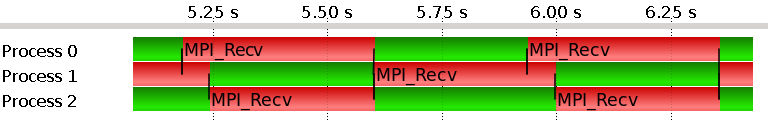
\includegraphics[scale=0.8]{gaussseidel-3-2-sync.png}
\caption{Sync-Übersicht}
\end{figure}

Gut erkennbar ist die Pipeline. Dadurch, dass die Synchronisation so viel
Zeit in Anspruch nimmt, kommt das Schachbrettmuster zustande.

\begin{figure}[H]
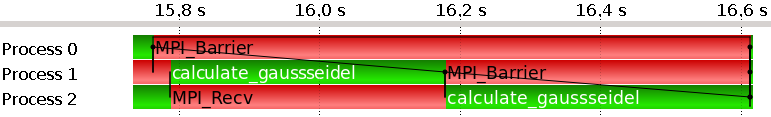
\includegraphics[scale=0.8]{gaussseidel-3-2-end.png}
\caption{Ende des Programms}
\end{figure}

Die Barriere sorgt dafür, dass die Pipeline korrekt ausläuft.

\begin{figure}[H]
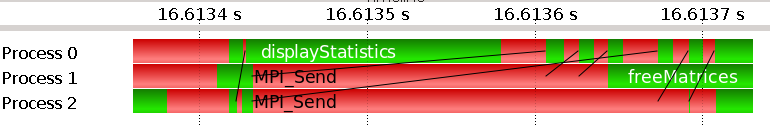
\includegraphics[scale=0.8]{gaussseidel-3-2-end2.png}
\caption{Closeup vom Ende}
\end{figure}

Gauss-Seidel und Jacobi verhalten sich beim Einsammeln der Ergebnisdaten
genau gleich.

\subsection{5 Prozesse, 4 Knoten}
\begin{figure}[H]
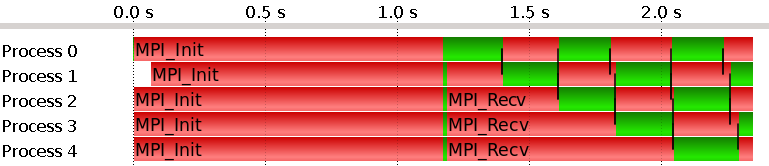
\includegraphics[scale=0.8]{gaussseidel-5-4-start.png}
\caption{Beginn des Programms}
\end{figure}
Das MPI\_Init verbraucht hier um die 1.25 Sekunden pro Prozess. Bei Process 1
fängt es etwas später an, was damit zu tun haben kann, dass einige Knoten zu
Schlafen beginnen, wenn sie länger nicht benutzt werden. Es kann auch damit zu
tun haben, dass in diesem Fall 2 Prozesse auf dem gleichen Knoten ausgeführt
werden.

\begin{figure}[H]
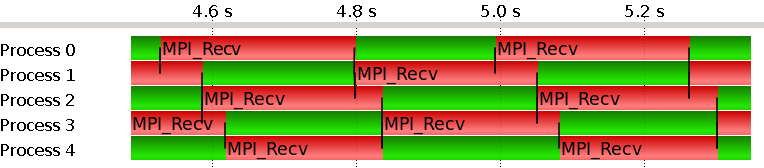
\includegraphics[scale=0.8]{gaussseidel-5-4-sync.png}
\caption{Sync-Übersicht}
\end{figure}

Wieder kann man alle Phänomene mit mehr Prozessen sehen.

\begin{figure}[H]
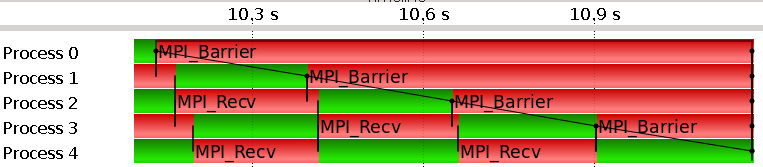
\includegraphics[scale=0.8]{gaussseidel-5-4-endbarrier.png}
\caption{Barriere kurz vor Ende}
\end{figure}

\begin{figure}[H]
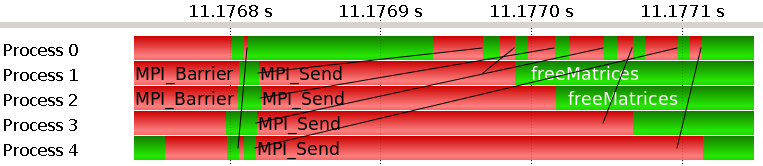
\includegraphics[scale=0.8]{gaussseidel-5-4-end.png}
\caption{Ende des Programms}
\end{figure}

\end{document}